\documentclass[12pt]{article} 
\usepackage[pdftex]{graphics}
\usepackage[english]{babel}
\usepackage{graphicx}
\usepackage{float}
\usepackage{chngpage}
\usepackage{multirow, lscape}
\usepackage{multicol}
\usepackage{url}
\usepackage{color}
\usepackage{natbib}
\usepackage[bookmarks=true, bookmarksopen=true, linkcolor=webblue]{hyperref}
\usepackage[left=1in,top=1in,right=1in,bottom=1in,nohead]{geometry}
\usepackage{booktabs, multicol, multirow}
\renewcommand{\baselinestretch}{1.5} %This sets the line spacing, right now it is set at 1.5 spacing. 

\title{Intro to \LaTeX}
\author{James Martherus}

\begin{document}
\maketitle

LaTeX is a typesetting language that produces publication-quality documents, including tables, charts, and equations. If you are used to creating documents in a word processor like Word or Google Docs, LaTeX  will have a bit of a learning curve. However, once you find a style you like, creating additional documents in that style is very straightforward. My goal here is not to make you LaTeX  experts, but to convince you that LaTeX  is worth the time to learn and to give you a basic primer and some reference documents to help you in the future. \\

Advantages of \LaTeX:
\begin{itemize}
    \item Allows you to write out equations much faster than Word.
    \item Simple integration of really nice tables from R using stargazer and other packages
    \item .bib files allow you to automatically generate references in many different styles. 
    \item miscellaneous smaller advantages like automatically updating figure/table numbers, etc.
\end{itemize}

\section*{Setting up a \LaTeX  document}

The first thing you need to create a document using LaTeX  is a .tex file. Think of these like R scripts, they are the instructions you are giving to LaTeX. The first line of your .tex file tells LaTeX  what type of document you would like to create, using the \verb \documentclass{}  command. In this file, I am using the ``article'' format, which will work for most documents you create. 

Next, you'll have several \verb \usepackage{}  commands. Like R, LaTeX  uses packages to access additional functionality. For example, this document is using a package called \verb url , which (surprise) lets us insert clickable urls into our document. 
Next, you'll usually set up your title page. You'll see this document uses a \verb title{}  command as well as an \verb author{}  command. After setting the title and author, I use the \verb \maketitle  command to actually create the title page. 

Finally, you begin the main portion of your document using the \verb document environment. Notice that we have both a \verb \begin{document}  and an \verb \end{document} . You'll use lots of different environments like these, and each one requires a \verb \begin{}  command and an \verb \end{}  command. 

We could spend lots of time talking about different packages and how to make all sorts of different types of documents. I don't think that's a good use of your time at this point. My recommendation is to spend some time looking at LaTeX  templates, find one you like, and start using it. Once you're more comfortable with everything, you can start customizing. Rather than spend more time on this today, I want to show you a few things you'll want to know for your first year of grad school. 


\section*{Tables in \LaTeX}

You can create tables in LaTeX  using a \verb tabular  environment. Inside the tabular environment, you indicate columns using \&, and indicate the end of a row using \verb \\  . You can also insert horizontal lines using \verb \hline . This is hard to explain in words, so check out this simple example: \\


\begin{tabular}{|l|l|} 
\hline
Fruit & Color \\
\hline
Apples & Green \\
Strawberries & Red \\
Oranges & Orange \\
\hline
\end{tabular} \\

You may need to assemble a table from scratch like this from time to time, but there's several excellent R packages that will create LaTeX  tables for you. The next page includes some output of a table I created this week using the \verb stargazer  package. You definitely don't want to have to do that by hand... I'll show you the \verb stargazer  package later. 

\begin{table}[!htbp] \centering 
  \caption{Difference in Personal Norm Strength Between Republicans and Democrats} 
  \label{} 
\begin{tabular}{@{\extracolsep{5pt}}lcc} 
\\[-1.8ex]\hline 
\hline \\[-1.8ex] 
 & \multicolumn{2}{c}{\textit{Dependent variable:}} \\ 
\cline{2-3} 
\\[-1.8ex] & Leader & Oppressed \\ 
\\[-1.8ex] & (1) & (2)\\ 
\hline \\[-1.8ex] 
 Republican & 0.038$^{**}$ & $-$0.072$^{***}$ \\ 
  & (0.017) & (0.016) \\ 
  & & \\ 
 Age & 0.562$^{***}$ & 0.606$^{***}$ \\ 
  & (0.012) & (0.011) \\ 
  & & \\ 
\hline \\[-1.8ex] 
Observations & 1,523 & 1,515 \\ 
R$^{2}$ & 0.003 & 0.013 \\ 
Adjusted R$^{2}$ & 0.002 & 0.013 \\ 
Residual Std. Error & 0.338 (df = 1521) & 0.308 (df = 1513) \\ 
F Statistic & 4.766$^{**}$ (df = 1; 1521) & 20.239$^{***}$ (df = 1; 1513) \\ 
\hline 
\hline \\[-1.8ex] 
\textit{Note:}  & \multicolumn{2}{r}{$^{*}$p$<$0.1; $^{**}$p$<$0.05; $^{***}$p$<$0.01} \\ 
\end{tabular} 
\end{table} 

\section*{Figures in \LaTeX}

Inserting figures in LaTeX  is pretty straightforward. I've included some sample code below. You can refer to images using the labels assigned inside the \verb figure  environment using the \verb ref{}  command. Look at the butterfly in figure \ref{image-myimage}. If you move the figure around (such that it is now figure 2 or figure 3), the reference will automatically update to reflect the new position of the figure.

\begin{figure}[h]
\centering
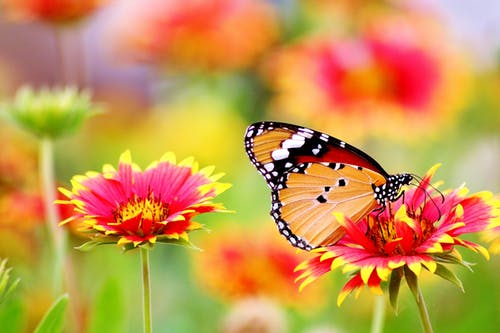
\includegraphics[width=.5\textwidth]{myimage.jpeg}
\caption{Here is a butterfly}
\label{image-myimage}
\end{figure}


\section*{Equations in \LaTeX}

You can easily write equations in LaTeX. To begin writing an equation, use the \$ or \$\$. A single \$ will put your equation ``inline'' meaning it will appear in your sentence. Here's what it looks like: $z = x + y$. A double \$\$ will put your equation on a different line and center it. Use this for larger equations:

$$ \frac{\sum\limits_{n}(x_{i} - \bar{x})(y_{i} - \bar{y})}{\sqrt{\sum\limits_{n}(x_{i} - \bar{x})^{2}}\sqrt{\sum\limits_{n}(y_{i} - \bar{y})^{2}}} = \frac{Cov[X,Y]}{SD[X] SD[Y]} $$ \\

There are several commands you'll use a lot when writing equations:

\begin{itemize}
    \item \verb \frac{}{}  gives you a fraction where the numerator goes in the first set of brackets and the denominator goes in the second set.
    \item \verb \sum  gives you the $\sum$ symbol.
    \item \verb _{}  will insert a subscript where the contents of the subscript are inside the brackets.
    \item \verb ^{}  does the same for a superscript.
    \item \verb \hat{}  puts a hat on the contents of the brackets, e.g., $\hat{x}$.
\end{itemize}

There are many more commands for making equations. Usually you'll easily find what you need by Googling, e.g., ``latex square root.'' 

\section*{Miscellaneous information}

You can \textbf{change} \textsc{how} \underline{your} \textit{text} looks or make it {\huge big} or {\tiny small}.

% You can also include comments to yourself using the the percentage symbol. These are ignored when you compile your document, so they show up in the .tex file, but not the .pdf. I use these sometimes if I'm not sure whether I want to keep a paragraph in a paper. 

\section*{Quick Reference Pages with .bib  Files}

Apart from your \verb .tex  file, the other really important file you'll want is a \verb .bib  file. These files include information about each book or article you cite, and LaTeX  uses them to compile your references page as well as insert references into your text.

Inserting references into the text is very simple. First, make sure you include the \verb natbib  package at the beginning of your document (insert this line: \verb \usepackage{natbib} ). Then, make sure you have these two commands near the end of your document (but before the \verb end{document}  command: First, use \verb \bibliographystyle{}  to tell LaTeX  how you want the references cited. Then use the \verb \bibliography{}  command with the name of your bib file in the brackets.

Finally, use one of the following commands:

\begin{itemize}
    \item \verb citet{}  to include the authors name in text with the year in parentheses.
    \item \verb citep{}  to include the name and year in parentheses.
\end{itemize}

Here's some examples: Here I'm citing \citet{Converse1964}, and here I'm citing something he said \citep{Converse1964}. Even though my .bib file has a ton of different references in it, only the ones I actually cite end up in the references page! You can also include other text in the citation using square brackets. Anything in the first square brackets will go before the reference, and anything in second pair will go after. For example, here i'm citing a page number \citep[][pg. 3]{levendusky:2018} and here i'm giving a list of examples \citep[e.g., see][]{schlesinger:1985, mason:2016, iyengar:2014}

You can create the entries for your .bib file by hand, but it takes a while and sort of defeats the purpose of trying to use these tools to save yourself time and effort. Tomorrow, we'll talk about reference management software and how to generate .bib files really easily. 

\section*{Conclusion}

There is a ton more that LaTeX  can do, but this brief tutorial should give you everything you need for your first year of grad school. I hope this file and the template file are resources you can return to during the year. For more in-depth coverage of some of these concepts, see \href{http://www.docs.is.ed.ac.uk/skills/documents/3722/3722-2014.pdf}{LaTeX for Beginners} and \href{https://www.latex-tutorial.com/tutorials/}{latex-tutorial.com}. 


\newpage
\bibliographystyle{apalike}
\bibliography{example.bib}

\end{document}